\documentclass{article}
\usepackage[utf8]{inputenc}
\usepackage[hidelinks]{hyperref}
\usepackage[a4paper]{geometry}
\usepackage{amssymb}
\usepackage{graphicx}
\usepackage{fancyhdr}
\usepackage{titlesec}
\usepackage{amsmath}

\titleformat*{\section}{\LARGE\bfseries}
\titleformat*{\subsection}{\Large\bfseries}

\pagestyle{fancy}

\lhead{\leftmark}
\rhead{Page \thepage}
\cfoot{Ojas Karanjkar 210070040}
\renewcommand{\footrulewidth}{1pt}

\begin{document}

\begin{titlepage}
\begin{center}
    \vspace*{\fill}
\includegraphics[scale=0.4]{iitb.png}\\
[4 cm]
    \rule{12.5cm}{0.75mm}\\
    \huge{\bfseries Filter Design Assignment}
    \rule{12.5cm}{0.75mm}\\
    [0.5cm]
   {\textbf {EE338 - 2023 \\
   FIR Filter Design Report}}\\
    [2.5cm]
\end{center}
\begin{flushleft}
   {\huge
    Ojas Karanjkar \\
    210070040 \\
     \\}
    \end{flushleft}
\end{titlepage}
\tableofcontents
\thispagestyle{empty}
\clearpage
\pagenumbering{arabic}

\newpage

\section{Student Details}
\begin{itemize}
    \item Name : Ojas Karanjkar
    \item Roll No: 210070040
    \item Filter number assigned: 103
\end{itemize}


\section{FIR Bandpass Filter}

\subsection{Un-normailzed Discrete time specifications}

\begin{itemize}
    \item \begin{enumerate}
                \item m = 23
                \item q(m) = [2.3] = 2
                \item r(m) = 23 - 10*2 = 3
                \item BL(m) = 20 + 3*2 + 11*3 = 59
                \item BH(m) = 59 + 75 = 134
            \end{enumerate}

    \item Passband = $59$ kHz to $134$ kHz.
    \item Transition Band Width = $5$ kHz.
    \item Stopband = $0$ to $54$ kHz and $139$ to $300$ kHz.
    \item Tolerance = 0.15.
    \item Nature of Passband = Equiripple.
    \item Nature of Stopband = Equiripple.
\end{itemize}


\subsection{Normailzed discrete filter specifications}
Sampling frequency = $600 kHz$\\
\begin{equation}
    \omega = \frac{\Omega * 2\pi}{\Omega _{sampling}}\\
\end{equation}

\begin{itemize}
    \item Passband = $0.1967\pi$ to $0.4467\pi$ .
    \item Transition Band Width = $0.0167\pi$ .
    \item Stopband = $0$ to $0.18$  and $0.4633\pi$ to $\pi$ .
    \item Tolerance = 0.15.
    \item Nature of Passband = Equiripple.
    \item Nature of Stopband = Equiripple.
\end{itemize}

Next, we calaculate the cutoff frequency for ideal lowpass filter by averaging the stopband and passband frequency at both the edges. Thus, we get two cutoff frequencies.

\begin{equation}
    f_{c1} = \frac{f_{s1} + f_{p1}}{2} = 56.5 kHz
\end{equation}

\begin{equation}
    f_{c2} = \frac{f_{s2} + f_{p1}}{2} = 136.5 kHz
\end{equation}

This can be converted to angular frequencies in the following way:
\begin{equation}
    \omega_{c1} = \frac{2\pi f_{c1}}{f_{sampling}} = 0.5917
\end{equation}

\begin{equation}
    \omega_{c2} = \frac{2\pi f_{c2}}{f_{sampling}} = 1.4294
\end{equation}


Next, we calculate $\omega_{T}$ required in the calculation of \textbf{N}.
\begin{equation}
    \omega_{T} = \frac{2\pi(Transition Band Width)}{f_{sampling}} = 0.01667\pi
\end{equation}


\subsection{Calculation of N for the FIR Bandpass Filter}

To determine the parameter $\beta$ which is used in generating the Kaiser Window function, we first calculate the attenuation A given by the following formula:

\begin{equation}
    A = -20log(Delta) = -20log(0.15) = 16.4782
\end{equation}

Now, as A is less than 21, we get $\beta$ = 0 which corresponds to rectangular window function.

Next, we calculate \textbf{N} for the Specifications of the Bandpass filter that I need to design using the following Empirical formula:- 

\[N = \lceil \frac{A - 7.95}{2.285*\omega_{T}} \rceil = 72\]

We now evaluate the FIR impulse response in the following sections for N points, N/2 points symmetrically around the origin.

To find the impulse response of bandpass filter, we subtract the impulse response of two lowpass filters, one whose cutoff frequency is $\omega_{c1}$ and other whose cutoff frequency is $\omega_{c2}$. \\
The impulse response for ideal lowpass filter is as follows:-

\begin{equation}
    h[n] = \frac{sin(\omega_{c}n)}{\pi n} if n \neq 0
\end{equation}
\begin{equation}
    h[0] = \frac{\omega_{c}}{\pi}
\end{equation}

Now, to find the coefficients of the \textbf{FIR Bandpass Filter} using the window approach, we use the following formula to get the coefficients:-

\[h_{FIR,BPF}[n] = h_{ideal,BPF}[n]*kaiserWindow[n]\]

Next, I plotted the frequency response and magnitude plot using the inbuilt functions in MATLAB.

\subsection{Magnitude and Frequency Response}
\begin{center}
    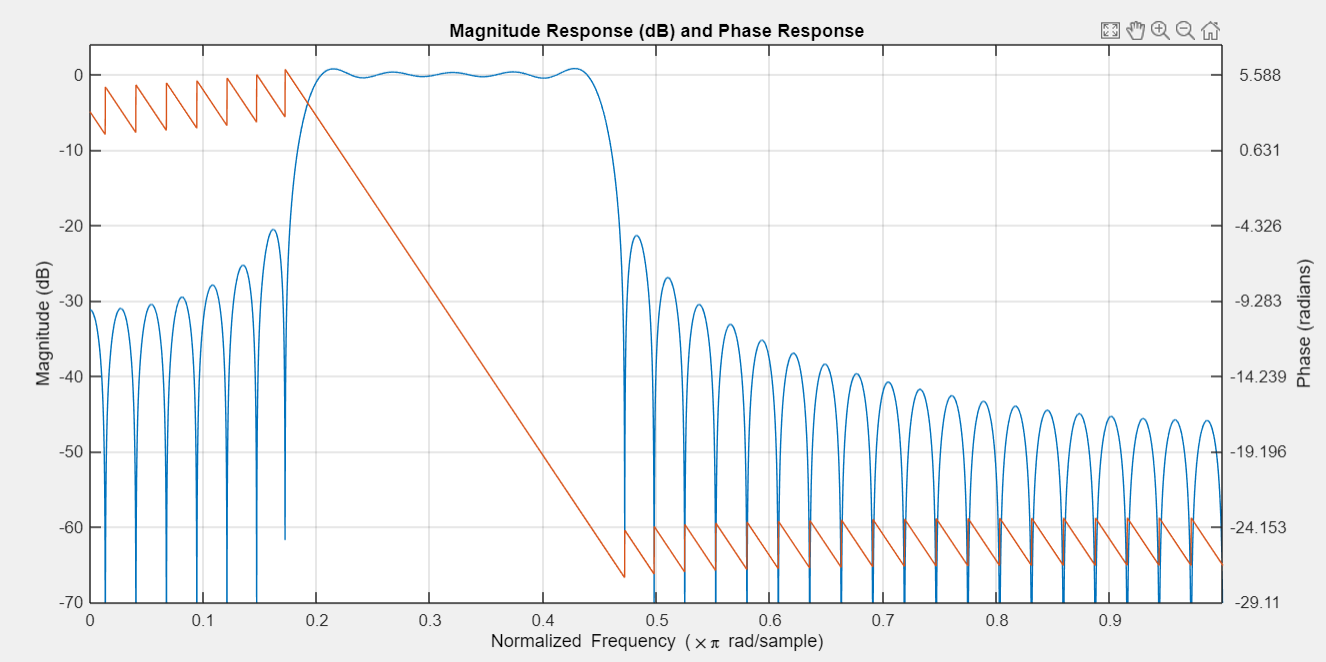
\includegraphics[scale=0.45]{bp_fir_mag.png}\\
    Frequency Response
\end{center}

\begin{center}
    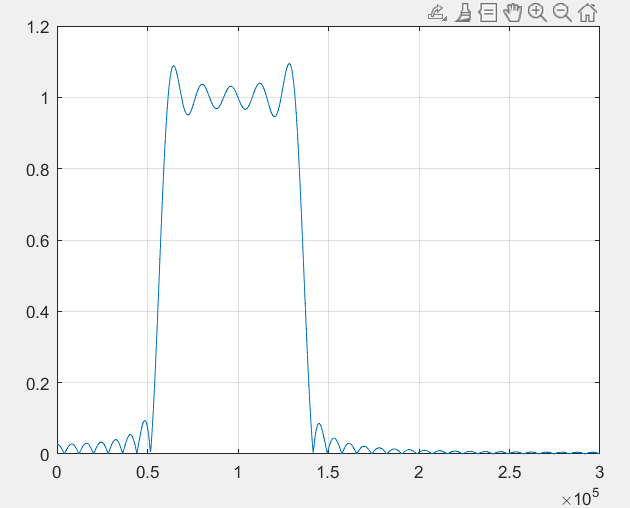
\includegraphics[scale=0.75]{bp_fir_magn.png}\\
    Magnitude plot
\end{center}

\newpage

\section{FIR Bandstop Filter}

\subsection{Un-normailzed Discrete time specifications}

\begin{itemize}
    \item \begin{enumerate}
                \item m = 23
                \item q(m) = [2.3] = 2
                \item r(m) = 23 - 10*2 = 3
                \item BL(m) = 20 + 3*2 + 11*3 = 59
                \item BH(m) = 59 + 40 = 99
            \end{enumerate}

    \item Stopband = $59$ kHz to $99$ kHz.
    \item Transition Band Width = $5$ kHz.
    \item Passband = $0$ to $54$ kHz and $104$ to $212.5$ kHz.
    \item Tolerance = 0.15.
    \item Nature of Passband and Stopband : Both equiripple.
\end{itemize}


\subsection{Normailzed discrete filter specifications}
Sampling frequency = $425 kHz$\\
\begin{equation}
    \omega = \frac{\Omega * 2\pi}{\Omega _{sampling}}\\
\end{equation}

\begin{itemize}
    \item Stopband = $0.27\pi$ to $0.46\pi$ .
    \item Transition Band Width = $0.0235\pi$ .
    \item Passband = $0$ to $0.25$  and $0.48\pi$ to $\pi$ .
    \item Tolerance = 0.15.
    \item Nature of Passband and Stopband : Both equiripple.
\end{itemize}


Next, we calaculate the cutoff frequency for ideal lowpass filter by averaging the stopband and passband frequency at both the edges. Thus, we get two cutoff frequencies.

\begin{equation}
    f_{c1} = \frac{f_{s1} + f_{p1}}{2} = 56.5 kHz
\end{equation}

\begin{equation}
    f_{c2} = \frac{f_{s2} + f_{p1}}{2} = 101.5 kHz
\end{equation}

This can be converted to angular frequencies in the following way:
\begin{equation}
    \omega_{c1} = \frac{2\pi f_{c1}}{f_{sampling}} = 0.8353
\end{equation}

\begin{equation}
    \omega_{c2} = \frac{2\pi f_{c2}}{f_{sampling}} = 1.5006
\end{equation}


Next, we calculate $\omega_{T}$ required in the calculation of \textbf{N}.
\begin{equation}
    \omega_{T} = \frac{2\pi(Transition Band Width)}{f_{sampling}} = 0.0235\pi
\end{equation}


\subsection{Calculation of N for the FIR Bandstop Filter}

To determine the parameter $\beta$ which is used in generating the Kaiser Window function, we first calculate the attenuation A given by the following formula:

\begin{equation}
    A = -20log(Delta) = -20log(0.15) = 16.4782
\end{equation}

Now, as A is less than 21, we get $\beta$ = 0 which corresponds to rectangular window function.

Next, we calculate \textbf{N} for the Specifications of the Bandstop filter that I need to design using the following Empirical formula:- 

\[N = \lceil \frac{A - 7.95}{2.285*\omega_{T}} \rceil = 51\]

We now evaluate the FIR impulse response in the following sections for N points, the origin and (N-1)/2 points symmetrically around the origin.

To find the impulse response of bandstop filter, we subtract the impulse response of two lowpass filters, one whose cutoff frequency is $\omega_{c2}$ from the impulse response of an all pass filter and add the impulse response of ideal lowpass filter whose cutoff frequency is $\omega_{c1}$. \\
The impulse response for ideal lowpass filter is as follows:-

\begin{equation}
    h[n] = \frac{sin(\omega_{c}n)}{\pi n} if n \neq 0
\end{equation}
\begin{equation}
    h[0] = \frac{\omega_{c}}{\pi}
\end{equation}

Now, to find the coefficients of the \textbf{FIR Bandstop Filter} using the window approach, we use the following formula to get the coefficients:-

\[h_{FIR,BSF}[n] = h_{ideal,BSF}[n]*kaiserWindow[n]\]

Next, I plotted the frequency response and magnitude plot using the inbuilt functions in MATLAB.

\subsection{Magnitude and Frequency Response}
\begin{center}
    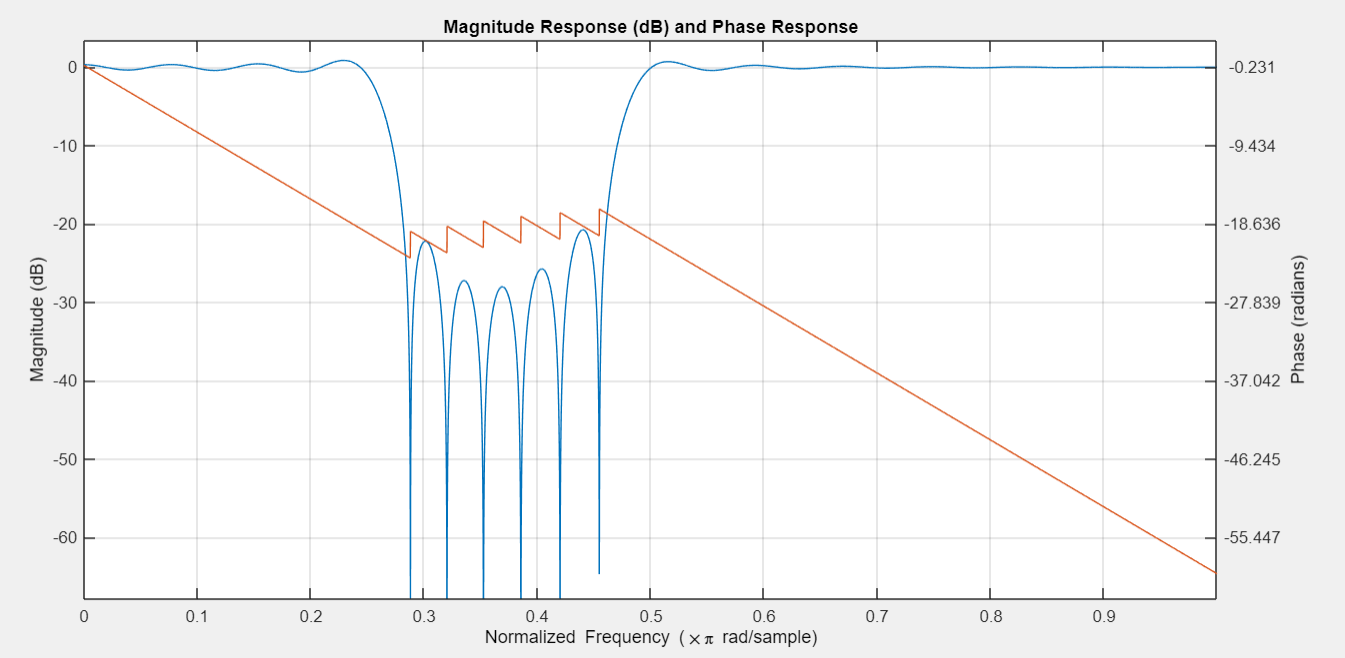
\includegraphics[scale=0.45]{bs_freq_fir.png}\\
    Frequency Response
\end{center}

\begin{center}
    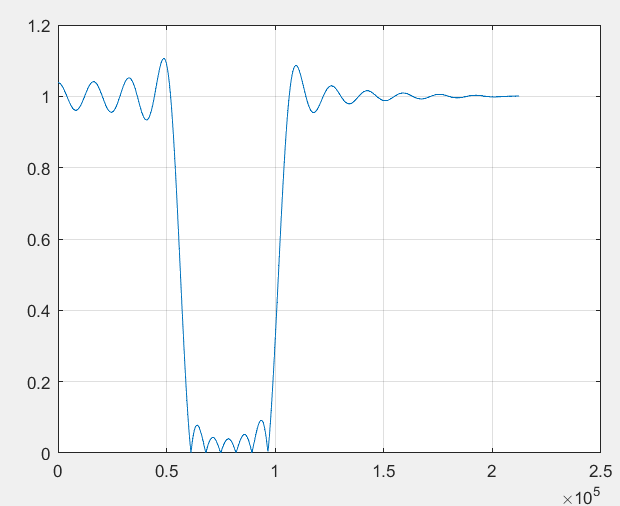
\includegraphics[scale=0.75]{bs_mag_fir.png}\\
    Magnitude plot
\end{center}
\newpage

\section{Comparison between FIR and IIR Realizations}
the major distinction between FIR and IIR filters is that IIR filters have Impulse responses that are non-zero for an infinite number of indexes, whereas FIR filters only have non-zero Impulse responses for a finite range of indices. Also, we can easily control the the specifications of FIR filter by simply changing the window length. In FIR filter, we can delay the output such that the impulse response is causal. Whereas, IIR filter is non-causal and we cannot introduce any delay in it. Also the transfer function of FIR filter only has zeros while IIR filter transfer function cna have both poles as well as zeros.

\section{Peer Review}

I have reviewed the FIR filter design of Kushal Gajbe, Roll No. 210070048. He has correctly found the frequency and magnitude response of the FIR filter and all the parameters are correct as well. Hence, I certify his FIR filter design to be correct.



\end{document}
